% Options for packages loaded elsewhere
\PassOptionsToPackage{unicode}{hyperref}
\PassOptionsToPackage{hyphens}{url}
%
\documentclass[
]{article}
\usepackage{amsmath,amssymb}
\usepackage{iftex}
\ifPDFTeX
  \usepackage[T1]{fontenc}
  \usepackage[utf8]{inputenc}
  \usepackage{textcomp} % provide euro and other symbols
\else % if luatex or xetex
  \usepackage{unicode-math} % this also loads fontspec
  \defaultfontfeatures{Scale=MatchLowercase}
  \defaultfontfeatures[\rmfamily]{Ligatures=TeX,Scale=1}
\fi
\usepackage{lmodern}
\ifPDFTeX\else
  % xetex/luatex font selection
\fi
% Use upquote if available, for straight quotes in verbatim environments
\IfFileExists{upquote.sty}{\usepackage{upquote}}{}
\IfFileExists{microtype.sty}{% use microtype if available
  \usepackage[]{microtype}
  \UseMicrotypeSet[protrusion]{basicmath} % disable protrusion for tt fonts
}{}
\makeatletter
\@ifundefined{KOMAClassName}{% if non-KOMA class
  \IfFileExists{parskip.sty}{%
    \usepackage{parskip}
  }{% else
    \setlength{\parindent}{0pt}
    \setlength{\parskip}{6pt plus 2pt minus 1pt}}
}{% if KOMA class
  \KOMAoptions{parskip=half}}
\makeatother
\usepackage{xcolor}
\usepackage{color}
\usepackage{fancyvrb}
\newcommand{\VerbBar}{|}
\newcommand{\VERB}{\Verb[commandchars=\\\{\}]}
\DefineVerbatimEnvironment{Highlighting}{Verbatim}{commandchars=\\\{\}}
% Add ',fontsize=\small' for more characters per line
\newenvironment{Shaded}{}{}
\newcommand{\AlertTok}[1]{\textcolor[rgb]{1.00,0.00,0.00}{\textbf{#1}}}
\newcommand{\AnnotationTok}[1]{\textcolor[rgb]{0.38,0.63,0.69}{\textbf{\textit{#1}}}}
\newcommand{\AttributeTok}[1]{\textcolor[rgb]{0.49,0.56,0.16}{#1}}
\newcommand{\BaseNTok}[1]{\textcolor[rgb]{0.25,0.63,0.44}{#1}}
\newcommand{\BuiltInTok}[1]{\textcolor[rgb]{0.00,0.50,0.00}{#1}}
\newcommand{\CharTok}[1]{\textcolor[rgb]{0.25,0.44,0.63}{#1}}
\newcommand{\CommentTok}[1]{\textcolor[rgb]{0.38,0.63,0.69}{\textit{#1}}}
\newcommand{\CommentVarTok}[1]{\textcolor[rgb]{0.38,0.63,0.69}{\textbf{\textit{#1}}}}
\newcommand{\ConstantTok}[1]{\textcolor[rgb]{0.53,0.00,0.00}{#1}}
\newcommand{\ControlFlowTok}[1]{\textcolor[rgb]{0.00,0.44,0.13}{\textbf{#1}}}
\newcommand{\DataTypeTok}[1]{\textcolor[rgb]{0.56,0.13,0.00}{#1}}
\newcommand{\DecValTok}[1]{\textcolor[rgb]{0.25,0.63,0.44}{#1}}
\newcommand{\DocumentationTok}[1]{\textcolor[rgb]{0.73,0.13,0.13}{\textit{#1}}}
\newcommand{\ErrorTok}[1]{\textcolor[rgb]{1.00,0.00,0.00}{\textbf{#1}}}
\newcommand{\ExtensionTok}[1]{#1}
\newcommand{\FloatTok}[1]{\textcolor[rgb]{0.25,0.63,0.44}{#1}}
\newcommand{\FunctionTok}[1]{\textcolor[rgb]{0.02,0.16,0.49}{#1}}
\newcommand{\ImportTok}[1]{\textcolor[rgb]{0.00,0.50,0.00}{\textbf{#1}}}
\newcommand{\InformationTok}[1]{\textcolor[rgb]{0.38,0.63,0.69}{\textbf{\textit{#1}}}}
\newcommand{\KeywordTok}[1]{\textcolor[rgb]{0.00,0.44,0.13}{\textbf{#1}}}
\newcommand{\NormalTok}[1]{#1}
\newcommand{\OperatorTok}[1]{\textcolor[rgb]{0.40,0.40,0.40}{#1}}
\newcommand{\OtherTok}[1]{\textcolor[rgb]{0.00,0.44,0.13}{#1}}
\newcommand{\PreprocessorTok}[1]{\textcolor[rgb]{0.74,0.48,0.00}{#1}}
\newcommand{\RegionMarkerTok}[1]{#1}
\newcommand{\SpecialCharTok}[1]{\textcolor[rgb]{0.25,0.44,0.63}{#1}}
\newcommand{\SpecialStringTok}[1]{\textcolor[rgb]{0.73,0.40,0.53}{#1}}
\newcommand{\StringTok}[1]{\textcolor[rgb]{0.25,0.44,0.63}{#1}}
\newcommand{\VariableTok}[1]{\textcolor[rgb]{0.10,0.09,0.49}{#1}}
\newcommand{\VerbatimStringTok}[1]{\textcolor[rgb]{0.25,0.44,0.63}{#1}}
\newcommand{\WarningTok}[1]{\textcolor[rgb]{0.38,0.63,0.69}{\textbf{\textit{#1}}}}
\usepackage{graphicx}
\makeatletter
\def\maxwidth{\ifdim\Gin@nat@width>\linewidth\linewidth\else\Gin@nat@width\fi}
\def\maxheight{\ifdim\Gin@nat@height>\textheight\textheight\else\Gin@nat@height\fi}
\makeatother
% Scale images if necessary, so that they will not overflow the page
% margins by default, and it is still possible to overwrite the defaults
% using explicit options in \includegraphics[width, height, ...]{}
\setkeys{Gin}{width=\maxwidth,height=\maxheight,keepaspectratio}
% Set default figure placement to htbp
\makeatletter
\def\fps@figure{htbp}
\makeatother
\ifLuaTeX
  \usepackage{luacolor}
  \usepackage[soul]{lua-ul}
\else
  \usepackage{soul}
\fi
\setlength{\emergencystretch}{3em} % prevent overfull lines
\providecommand{\tightlist}{%
  \setlength{\itemsep}{0pt}\setlength{\parskip}{0pt}}
\setcounter{secnumdepth}{-\maxdimen} % remove section numbering
\ifLuaTeX
  \usepackage{selnolig}  % disable illegal ligatures
\fi
\IfFileExists{bookmark.sty}{\usepackage{bookmark}}{\usepackage{hyperref}}
\IfFileExists{xurl.sty}{\usepackage{xurl}}{} % add URL line breaks if available
\urlstyle{same}
\hypersetup{
  pdftitle={Renato Ramirez},
  hidelinks,
  pdfcreator={LaTeX via pandoc}}

\title{Renato Ramirez}
\author{}
\date{}

\begin{document}
\maketitle

\subsection{Corne Keyboard by Foostan}\label{corne-keyboard-by-foostan}

\href{https://github.com/foostan/crkbd}{foostan/crkbd: Corne keyboard, a
split keyboard with 3x6 column staggered keys and 3 thumb keys.
(github.com)}

Flash tool : \href{https://qmk.fm/}{QMK Firmware - An open source
firmware for AVR and ARM based keyboards}\\
Chip : \href{https://www.sparkfun.com/products/12640}{Pro Micro -
5V/16MHz - DEV-12640 - SparkFun Electronics}\\
Firmware
:\href{https://github.com/foostan/crkbd/blob/main/doc/firmware_en.md}{crkbd/doc/firmwarefoostan/crkbd}\\
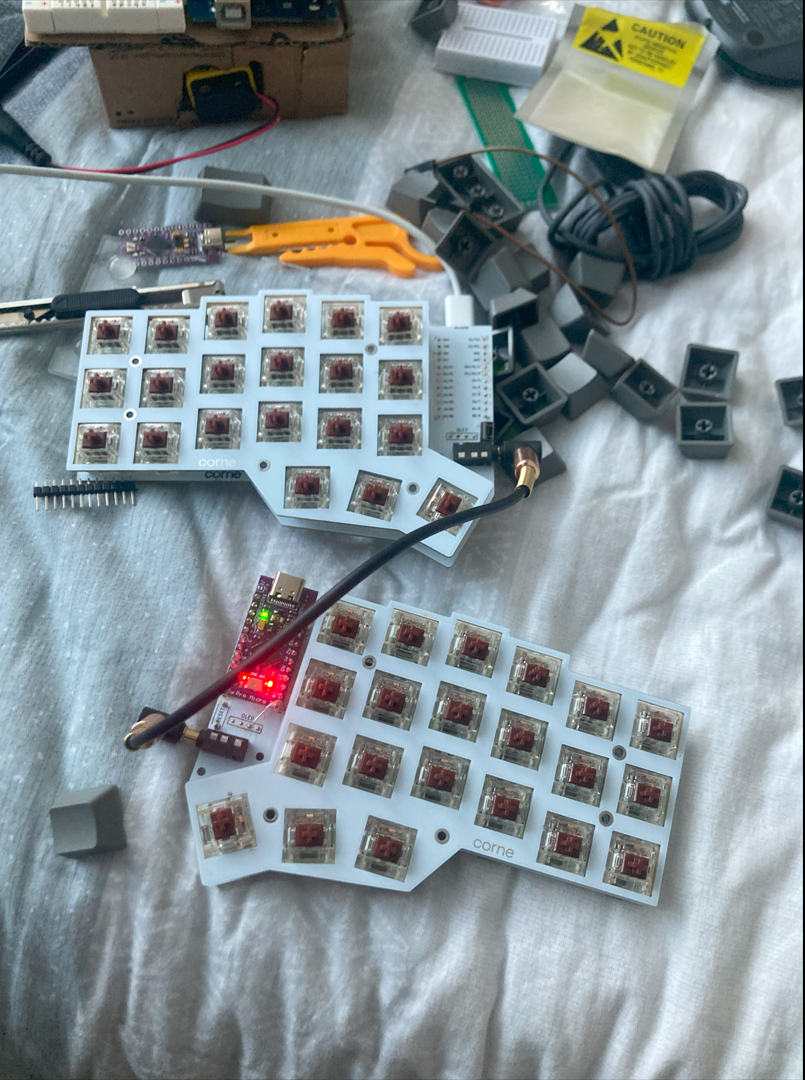
\includegraphics{C:/Users/capi_/OneDrive/Documents/MEGAsync/RenaplexMain/Screenshot 2023-10-20 105815.png}\\
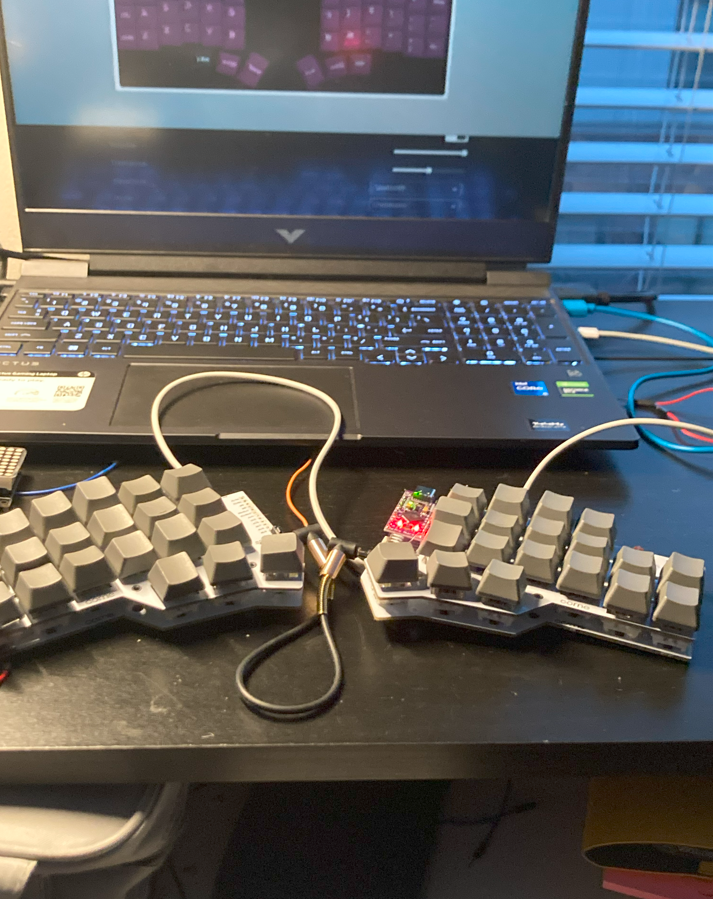
\includegraphics{C:/Users/capi_/OneDrive/Documents/MEGAsync/RenaplexMain/Screenshot 2023-10-20 105723.png}\\
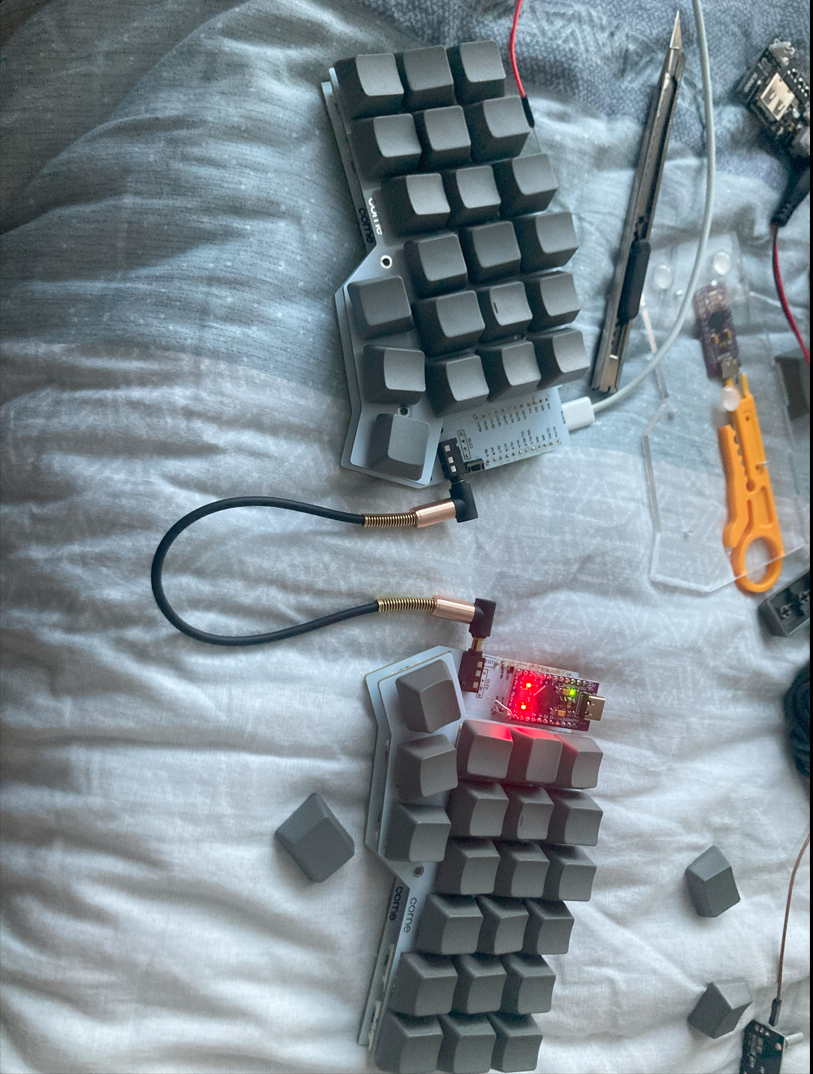
\includegraphics{C:/Users/capi_/OneDrive/Documents/MEGAsync/RenaplexMain/Screenshot 2023-10-20 105801.png}

\begin{center}\rule{0.5\linewidth}{0.5pt}\end{center}

\subsection{MAX7219 Led Module \& Fan led
control}\label{max7219-led-module-fan-led-control}

Board:
\href{https://store.arduino.cc/products/arduino-mega-2560-rev3}{Arduino
Mega 2560 Rev3}\\
Modules:
\href{https://projecthub.arduino.cc/mdraber/controlling-8x8-dot-matrix-with-max7219-and-arduino-0c417a}{Max7219}

\begin{Shaded}
\begin{Highlighting}[]
\NormalTok{\#include "LedControl.h"}
\NormalTok{LedControl lc = LedControl(12, 10, 11, 1);}
\NormalTok{unsigned long tiempoEspera1 = 500;}
\NormalTok{unsigned long tiempoEspera2 = 50;}
\NormalTok{void setup() \{}
\NormalTok{  lc.shutdown(0, false);}
\NormalTok{  lc.setIntensity(0, 8);}
\NormalTok{  lc.clearDisplay(0);}
\NormalTok{\}}
\NormalTok{void escribirArduinoEnMatriz() \{}
\NormalTok{  byte t[5] = \{B11111110, B00001000, B00001000, B00001000, B00001000\};}
\NormalTok{  byte e[5] = \{B11111110, B10001010, B10001010, B10001010, B10000010\};}
\NormalTok{  byte x[5] = \{B10000010, B01000100, B00101000, B01000100, B10000010\};}
\NormalTok{  byte a[5] = \{B10001000, B01010100, B00100010, B01010100, B10001000\};}
\NormalTok{  byte s[5] = \{B10000100, B10001010, B10001010, B10001010, B01000100\};}
\NormalTok{  byte t2[5] = \{B00001000, B11111110, B10001000, B10001000, B01000000\};}
\NormalTok{  byte e2[5] = \{B11111110, B10001010, B10001010, B10001010, B10000010\};}
\NormalTok{  byte c[5] = \{B01111100, B10000010, B10000010, B10000010, B01000100\};}
\NormalTok{  byte h[5] = \{B11111110, B00001000, B00001000, B00001000, B11111110\};}
\NormalTok{  lc.setRow(0, 0, t[0]);}
\NormalTok{  lc.setRow(0, 1, t[1]);}
\NormalTok{  lc.setRow(0, 2, t[2]);}
\NormalTok{  lc.setRow(0, 3, t[3]);}
\NormalTok{  lc.setRow(0, 4, t[4]);}
\NormalTok{  delay(tiempoEspera1);}
\NormalTok{  lc.setRow(0, 0, e[0]);}
\NormalTok{  lc.setRow(0, 1, e[1]);}
\NormalTok{  lc.setRow(0, 2, e[2]);}
\NormalTok{  lc.setRow(0, 3, e[3]);}
\NormalTok{  lc.setRow(0, 4, e[4]);}
\NormalTok{  delay(tiempoEspera1);}
\NormalTok{  lc.setRow(0, 0, x[0]);}
\NormalTok{  lc.setRow(0, 1, x[1]);}
\NormalTok{  lc.setRow(0, 2, x[2]);}
\NormalTok{  lc.setRow(0, 3, x[3]);}
\NormalTok{  lc.setRow(0, 4, x[4]);}
\NormalTok{  delay(tiempoEspera1);}
\NormalTok{  lc.setRow(0, 0, a[0]);}
\NormalTok{  lc.setRow(0, 1, a[1]);}
\NormalTok{  lc.setRow(0, 2, a[2]);}
\NormalTok{  lc.setRow(0, 3, a[3]);}
\NormalTok{  lc.setRow(0, 4, a[4]);}
\NormalTok{  delay(tiempoEspera1);}
\NormalTok{  lc.setRow(0, 0, s[0]);}
\NormalTok{  lc.setRow(0, 1, s[1]);}
\NormalTok{  lc.setRow(0, 2, s[2]);}
\NormalTok{  lc.setRow(0, 3, s[3]);}
\NormalTok{  lc.setRow(0, 4, s[4]);}
\NormalTok{  delay(tiempoEspera1);}
\NormalTok{  lc.setRow(0, 0, t2[0]);}
\NormalTok{  lc.setRow(0, 1, t2[1]);}
\NormalTok{  lc.setRow(0, 2, t2[2]);}
\NormalTok{  lc.setRow(0, 3, t2[3]);}
\NormalTok{  lc.setRow(0, 4, t2[4]);}
\NormalTok{  delay(tiempoEspera1);}
\NormalTok{  lc.setRow(0, 0, e2[0]);}
\NormalTok{  lc.setRow(0, 1, e2[1]);}
\NormalTok{  lc.setRow(0, 2, e2[2]);}
\NormalTok{  lc.setRow(0, 3, e2[3]);}
\NormalTok{  lc.setRow(0, 4, e2[4]);}
\NormalTok{  delay(tiempoEspera1);}
\NormalTok{  lc.setRow(0, 0, c[0]);}
\NormalTok{  lc.setRow(0, 1, c[1]);}
\NormalTok{  lc.setRow(0, 2, c[2]);}
\NormalTok{  lc.setRow(0, 3, c[3]);}
\NormalTok{  lc.setRow(0, 4, c[4]);}
\NormalTok{  delay(tiempoEspera1);}
\NormalTok{  lc.setRow(0, 0, h[0]);}
\NormalTok{  lc.setRow(0, 1, h[1]);}
\NormalTok{  lc.setRow(0, 2, h[2]);}
\NormalTok{  lc.setRow(0, 3, h[3]);}
\NormalTok{  lc.setRow(0, 4, h[4]);}
\NormalTok{  delay(tiempoEspera1);}
\NormalTok{  lc.setRow(0, 0, 0);}
\NormalTok{  lc.setRow(0, 1, 0);}
\NormalTok{  lc.setRow(0, 2, 0);}
\NormalTok{  lc.setRow(0, 3, 0);}
\NormalTok{  lc.setRow(0, 4, 0);}
\NormalTok{  delay(tiempoEspera1);}
\NormalTok{\}}

\NormalTok{void filas() \{}
\NormalTok{  for (int fila = 0; fila \textless{} 8; fila++) \{}
\NormalTok{    delay(tiempoEspera2);}
\NormalTok{    lc.setRow(0, fila, B10100000);}
\NormalTok{    delay(tiempoEspera2);}
\NormalTok{    lc.setRow(0, fila, (byte)0);}
\NormalTok{    for (int i = 0; i \textless{} fila; i++) \{}
\NormalTok{      delay(tiempoEspera2);}
\NormalTok{      lc.setRow(0, fila, B10100000);}
\NormalTok{      delay(tiempoEspera2);}
\NormalTok{      lc.setRow(0, fila, (byte)0);}
\NormalTok{    \}}
\NormalTok{  \}}
\NormalTok{\}}
\NormalTok{void columnas() \{}
\NormalTok{  for (int columna = 0; columna \textless{} 8; columna++) \{}
\NormalTok{    delay(tiempoEspera2);}
\NormalTok{    lc.setColumn(0, columna, B00100000);}
\NormalTok{    delay(tiempoEspera2);}
\NormalTok{    lc.setColumn(0, columna, (byte)0);}
\NormalTok{    for (int i = 0; i \textless{} columna; i++) \{}
\NormalTok{      delay(tiempoEspera2);}
\NormalTok{      lc.setColumn(0, columna, B00100000);}
\NormalTok{      delay(tiempoEspera2);}
\NormalTok{      lc.setColumn(0, columna, (byte)0);}
\NormalTok{    \}}
\NormalTok{  \}}
\NormalTok{\}}
\NormalTok{void individuales() \{}
\NormalTok{  for (int fila = 0; fila \textless{} 8; fila++) \{}
\NormalTok{    for (int columna = 0; columna \textless{} 8; columna++) \{}
\NormalTok{      delay(tiempoEspera2);}
\NormalTok{      lc.setLed(0, fila, columna, true);}
\NormalTok{      delay(tiempoEspera2);}
\NormalTok{      for (int i = 0; i \textless{} columna; i++) \{}
\NormalTok{        lc.setLed(0, fila, columna, false);}
\NormalTok{        delay(tiempoEspera2);}
\NormalTok{        lc.setLed(0, fila, columna, true);}
\NormalTok{        delay(tiempoEspera2);}
\NormalTok{      \}}
\NormalTok{    \}}
\NormalTok{  \}}
\NormalTok{\}}
\NormalTok{void loop() \{}
\NormalTok{  escribirArduinoEnMatriz();}
\NormalTok{  filas();}
\NormalTok{  columnas();}
\NormalTok{  individuales();}
\NormalTok{\}}
\NormalTok{Copy}
\end{Highlighting}
\end{Shaded}

\includegraphics{C:/Users/capi_/OneDrive/Documents/MEGAsync/RenaplexMain/mood (1).png}

\includegraphics{C:/Users/capi_/OneDrive/Documents/MEGAsync/RenaplexMain/Pasted image 20231020111120.png}

\begin{center}\rule{0.5\linewidth}{0.5pt}\end{center}

\subsection{Temperature And TT}\label{temperature-and-tt}

Board:
\href{https://store.arduino.cc/products/arduino-mega-2560-rev3}{Arduino
Mega 2560 Rev3}

Modules :\\
-*LCD1602 módule\\
-Potentiometer (10k)

\begin{Shaded}
\begin{Highlighting}[]
\NormalTok{\#include \textless{}LiquidCrystal.h\textgreater{}}
\NormalTok{LiquidCrystal lcd(7, 8, 9, 10, 11, 12);}
\NormalTok{int pinTemp = 0;}
\NormalTok{int indicePantalla = 0;}
\NormalTok{long ultimoCambioPantalla = millis();}
\NormalTok{void mostrarMensaje1() \{}
\NormalTok{  lcd.clear();}
\NormalTok{  lcd.setCursor(0, 0);}
\NormalTok{  lcd.print("Temp         C  ");}
\NormalTok{  lcd.setCursor(6, 0);}
\NormalTok{  int lecturaTemp = analogRead(pinTemp);}
\NormalTok{  double tempK = log(10000.0 * ((1024.0 / lecturaTemp {-} 1)));}
\NormalTok{  tempK = 1 / (0.001129148 + (0.000234125 + (0.0000000876741 * tempK * tempK )) * tempK );}
\NormalTok{  float tempC = tempK {-} 273.15;}
\NormalTok{  lcd.print(tempC);}
\NormalTok{\}}
\NormalTok{void mostrarMensaje2() \{}
\NormalTok{  lcd.clear();}
\NormalTok{  lcd.setCursor(0, 0);}
\NormalTok{  lcd.print("TexasTech \textless{}3");}
\NormalTok{  lcd.setCursor(0, 1);}
\NormalTok{  lcd.print("Renato Ramirez");}
\NormalTok{\}}

\NormalTok{void cambiarPantallas() \{}
\NormalTok{  indicePantalla++;}
\NormalTok{  if (indicePantalla \textgreater{}= 2) \{}
\NormalTok{    indicePantalla = 0;}
\NormalTok{  \}}
\NormalTok{  mostrarMensaje(indicePantalla);}
\NormalTok{\}}
\NormalTok{void mostrarMensaje(int indice) \{}
\NormalTok{  switch (indice) \{}
\NormalTok{    case 0:}
\NormalTok{      mostrarMensaje1();}
\NormalTok{      break;}
\NormalTok{    case 1:}
\NormalTok{      mostrarMensaje2();}
\NormalTok{      break;}
\NormalTok{  \}}
\NormalTok{\}}

\NormalTok{void setup() \{}
\NormalTok{  lcd.begin(16, 2);}
\NormalTok{  mostrarMensaje1();}
\NormalTok{\}}
\NormalTok{void loop() \{}
\NormalTok{  long tiempoTranscurrido = millis() {-} ultimoCambioPantalla;}
\NormalTok{  if (tiempoTranscurrido \textgreater{}= 5000) \{}
\NormalTok{    cambiarPantallas();}
\NormalTok{    ultimoCambioPantalla = millis();}
\NormalTok{  \}}
\NormalTok{\}}
\NormalTok{Copy}
\end{Highlighting}
\end{Shaded}

\includegraphics{C:/Users/capi_/OneDrive/Documents/MEGAsync/RenaplexMain/Pasted image 20231020111335.png}\\
\includegraphics{C:/Users/capi_/OneDrive/Documents/MEGAsync/RenaplexMain/Pasted image 20231020111351.png}

\begin{center}\rule{0.5\linewidth}{0.5pt}\end{center}

\subsection{RFID access with Alarm
led}\label{rfid-access-with-alarm-led}

Modules: RFID RC522, Active Buzzer\\
Board: Arduino Mega 2560 v3

\begin{Shaded}
\begin{Highlighting}[]
\NormalTok{\#include \textless{}SPI.h\textgreater{}}
\NormalTok{\#include \textless{}RFID.h\textgreater{}}
\NormalTok{\#define SDA\_DIO 9}
\NormalTok{\#define RESET\_DIO 8}
\NormalTok{RFID RC522(SDA\_DIO, RESET\_DIO);}
\NormalTok{const int ledPin = 2;}
\NormalTok{void setup()}
\NormalTok{\{}
\NormalTok{  Serial.begin(9600);}
\NormalTok{  SPI.begin();}
\NormalTok{  RC522.init();}
\NormalTok{  pinMode(ledPin, OUTPUT);}
\NormalTok{  digitalWrite(ledPin, LOW);}
\NormalTok{\}}
\NormalTok{void loop()}
\NormalTok{\{}
\NormalTok{  if (RC522.isCard())}
\NormalTok{  \{}
\NormalTok{    RC522.readCardSerial();}
\NormalTok{    Serial.println("Card detected:");}
\NormalTok{    for (int i = 0; i \textless{} 5; i++)}
\NormalTok{    \{}
\NormalTok{      Serial.print(RC522.serNum[i], DEC);}
\NormalTok{    \}}
\NormalTok{    Serial.println();}
\NormalTok{    digitalWrite(ledPin, HIGH);}
\NormalTok{    String name;}
\NormalTok{    Serial.println("Please enter your name and press Enter:");}
\NormalTok{    while (Serial.available() == 0)}
\NormalTok{    \{}
\NormalTok{    \}}
\NormalTok{    while (Serial.available() \textgreater{} 0)}
\NormalTok{    \{}
\NormalTok{      char c = Serial.read();}
\NormalTok{      if (c == \textquotesingle{}\textbackslash{}n\textquotesingle{})}
\NormalTok{      \{}
\NormalTok{        break;}
\NormalTok{      \}}
\NormalTok{      name += c;}
\NormalTok{    \}}
\NormalTok{    Serial.println("Name saved: " + name);}
\NormalTok{    Serial.println()}
\NormalTok{    // Apaga la luz}
\NormalTok{    delay(2000);}
\NormalTok{    digitalWrite(ledPin, LOW);}
\NormalTok{  \}}
\NormalTok{\}}
\NormalTok{Copy}
\end{Highlighting}
\end{Shaded}

\textquotesingle\textquotesingle\textquotesingle{}\\
\includegraphics{C:/Users/capi_/OneDrive/Documents/MEGAsync/RenaplexMain/Pasted image 20231020112405.png}\\
\includegraphics{C:/Users/capi_/OneDrive/Documents/MEGAsync/RenaplexMain/Pasted image 20231020112329.png}\includegraphics{C:/Users/capi_/OneDrive/Documents/MEGAsync/RenaplexMain/Pasted image 20231020112453.png}\includegraphics{C:/Users/capi_/OneDrive/Documents/MEGAsync/RenaplexMain/Pasted image 20231020112509.png}

\subsection{Other programs I made and
Diplomas}\label{other-programs-i-made-and-diplomas}

This is a game I found a while ago. It\textquotesingle s one of the
first programs I made. It\textquotesingle s in Spanish and it
doesn\textquotesingle t work completely, haha. But it used to work.
Other programs I made were a \hl{proxy server}, and I also know how to
use \hl{Wireshark (software)}. It was very fun because in Venezuela, the
routers are very old and always outdated, so I could do some really
interesting things

\begin{Shaded}
\begin{Highlighting}[]
\NormalTok{import string}
\NormalTok{import random}

\NormalTok{vaul = ["MUEBLE", "BIBLIOTECA", "CAMALEON", "SINGAPUR", "SOFA", "ESTUDIANTE", "PROGRAMADOR", "CASTILLO", "TOPO"]}

\NormalTok{palabra = random.choice(vaul)}

\NormalTok{print("Welcome al juego del ahorcado")}

\NormalTok{print("Tu palabra tiene " + str(len(palabra)) + " letras!")}
  
\NormalTok{printeado = "\_ " * len(palabra)}
\NormalTok{n\_intentos = 6  \# Número de intentos permitidos}
\NormalTok{intentos = 0  \# Número de intentos realizados}

\NormalTok{while printeado != palabra and intentos \textless{} n\_intentos:}

\NormalTok{    user\_input = input("¿Qué letra quieres adivinar? ").upper()}
\NormalTok{    if len(user\_input) != 1 or user\_input not in string.ascii\_uppercase:}
\NormalTok{        print("Entrada inválida. Ingresa una sola letra en mayúscula.")}
\NormalTok{        continue}
\NormalTok{    if user\_input in palabra:}
\NormalTok{        for i in range(len(palabra)):}
\NormalTok{            if palabra[i] == user\_input:}
\NormalTok{                printeado = printeado[:i] + user\_input + printeado[i+1:]}
\NormalTok{    else:}
\NormalTok{        intentos += 1}
\NormalTok{        print("Lo siento, tu letra no está en la palabra. Te quedan \{\} intentos.".format(n\_intentos {-} intentos)}
\NormalTok{    print(printeado)}
\NormalTok{if printeado == palabra:}
\NormalTok{    print("¡Felicidades! Has adivinado la palabra: " + palabra)}

\NormalTok{else:}
\NormalTok{    print("Agotaste tus intentos. La palabra era: " + palabra)\textasciigrave{}\textasciigrave{}\textasciigrave{}}
\NormalTok{![[Pasted image 20231020115805.png]]}
\NormalTok{![[Pasted image 20231020115733.png]]}
\NormalTok{![[Pasted image 20231020115701.png]]![[Pasted image 20231020120152.png]]}





















\NormalTok{\#\# Rubik\textquotesingle{}s Cube and Drawing Skills}
\NormalTok{**I am a talented artist and also speedCuber, and I believe that my skills could be valuable in an extracurricular activity.**}

\NormalTok{Unfortunately, I can\textquotesingle{}t show you my large collection of Rubik\textquotesingle{}s Cubes. Most of them are in Venezuela, and my mother is keeping them for now. My collection was about 12 different types of cubes, from 3x3 to mirror. It is still one of my great passions, and I still practice. When I arrived in the United States, I was very excited, as the community is much larger here, and there are clubs and competitions frequently. Unfortunately, I got sick when I arrived, so I haven\textquotesingle{}t been able to go to any, but I eventually will. It is one of my dreams.}

\NormalTok{**2x2** :sub7}
\NormalTok{**3x3** :sub27}
\NormalTok{**4x4** :sub4m}
\NormalTok{**5x5**:no yet}
\NormalTok{**Megaminx**:sub8}
\NormalTok{**Pyraminx** :sub30}

\NormalTok{I know, a lot of people think I should study architecture. I like the idea quite a bit, but I think my place is at Edward E. Whitacre Jr. College.😉}
\NormalTok{![[Pasted image 20231020132857.png]]}
\NormalTok{![[Pasted image 20231020132832.png]]}
\NormalTok{![[Pasted image 20231020132755.png]]}
\NormalTok{![[Pasted image 20231020132741.png]]}

\NormalTok{![[Pasted image 20231020132728.png]]}





\NormalTok{Copy}
\end{Highlighting}
\end{Shaded}


\end{document}
